\documentclass{article}
\usepackage[UTF8]{ctex}
\usepackage{hyperref}
\usepackage{graphicx}
\usepackage{listings}
\usepackage{subfigure}
\usepackage{booktabs}
\usepackage{multirow}
\usepackage{placeins}
\usepackage{booktabs}
\usepackage{multirow} 
\usepackage{caption}
\usepackage{changepage} 
\usepackage{adjustbox} % 用于调整表格大小
\usepackage{geometry} % 用于调整页边距
\usepackage{amsmath}
\usepackage{amssymb}
\usepackage{natbib}
\usepackage{algorithm}
\usepackage{algorithmic}
\bibliographystyle{plain}


\title{使用细节增强网络和对抗式训练的去雾模型}
\author{作者:张林涛}
\date{2024 年 5 月 13 日}

\begin{document}

\maketitle

\begin{figure*}[t]
  \centering
  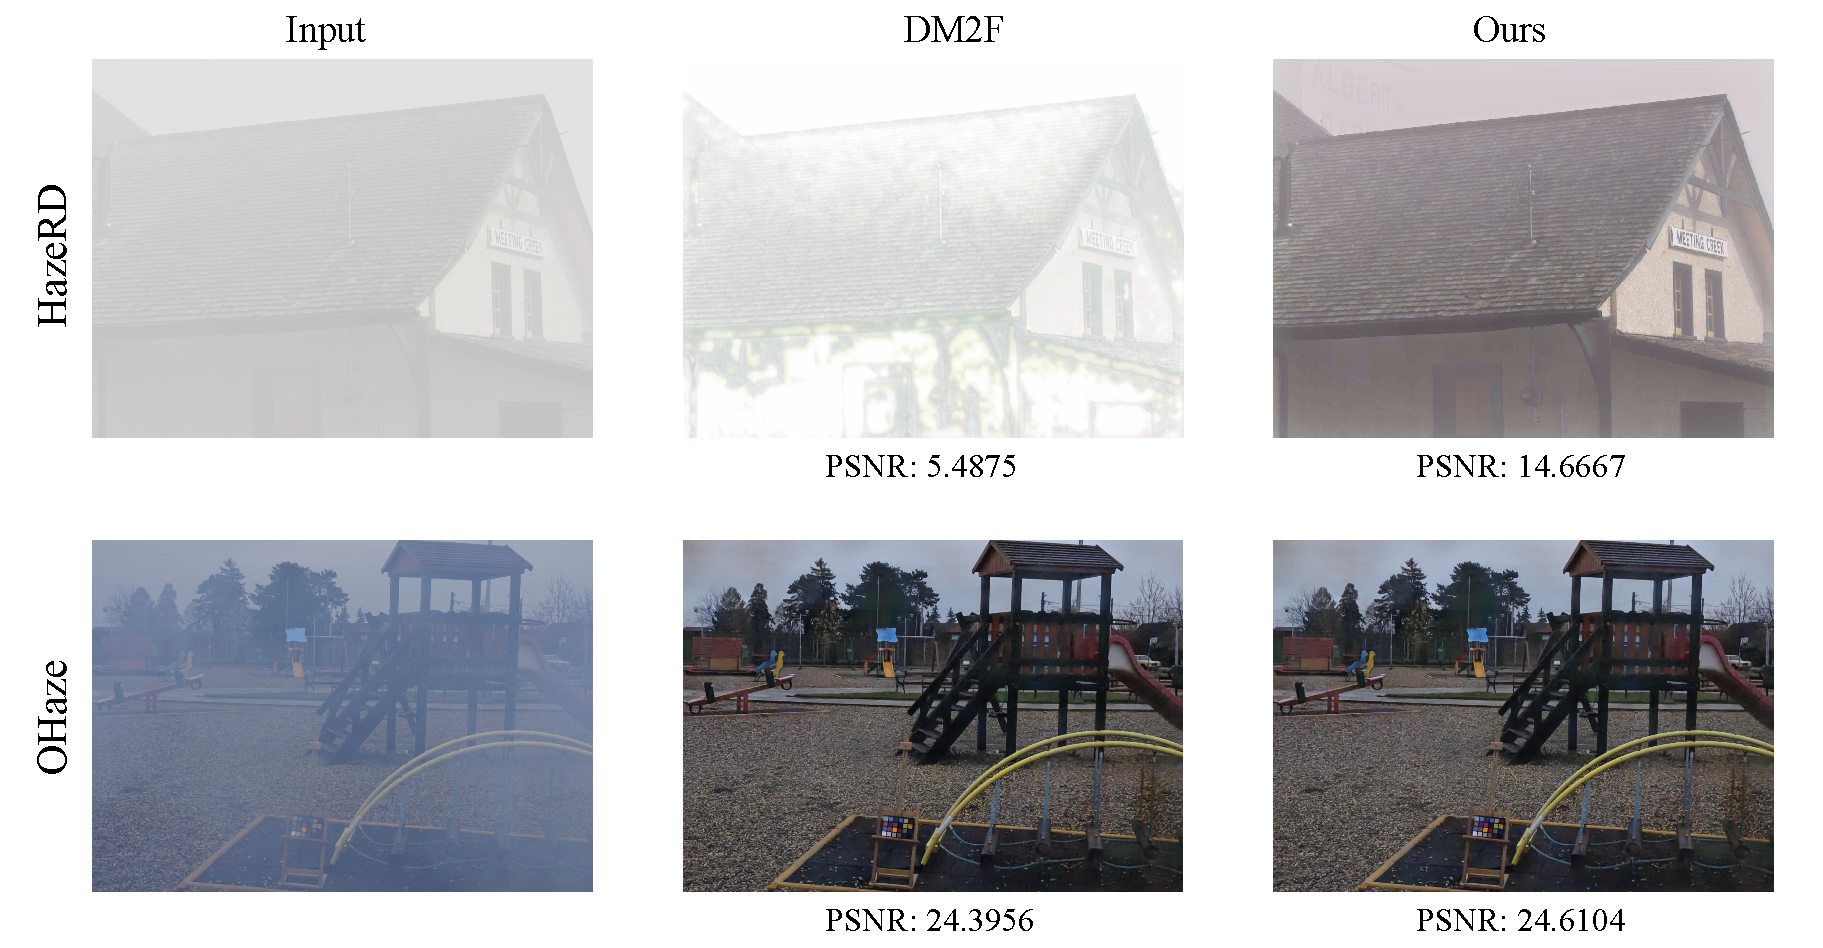
\includegraphics[width=.9\linewidth]{image/fig1.pdf}
  \caption{图像去雾效果对比}
  \label{fig:fig1}
\end{figure*}

\section{摘要}
% 超分辨率是指利用低分辨率图像生成高分辨率图像,获得更多的图像细节的视觉任务,当今大多数现有的方法针对特定的像素尺寸对进行训练,限制了其在不同分辨率下的泛化能力。在这篇论文中,我们提出了基于去噪扩散概率模型( DDPM )的超分方法,适用于不同尺寸的低分辨率输入。我们采用预训练的无条件DDPM作为生成式先验。我们只改变反向扩散迭代,利用原始图像作为信息控制上采样后图像的生成。通过该方法我们可以将一个模型应用于多个不同尺寸的超分任务,大大提高了模型的泛化能力。我们的方法在测试集上与SOTA模型效果接近。

单图像去雾任务指的是从单帧单目图像中恢复出高质量的清晰场景图像。Deng等人提出的基于深度学习的方法用注意力机制融合了多模型的特征,去雾效果超越了此前的单图像去雾算法,但仍存在恢复出的图像细节模糊、难以处理极端大雾情况等问题,如图~\ref{fig:fig1}所示。本文引入两种算法,分别解决了OHaze测试集上图像细节模糊和HazeRD测试集上极端大雾图像恢复效果差的问题。具体而言,为了修复模糊的图像细节,我们在原有模型的基础上引入了多色彩空间的细节增强网络,同时采用了高频低频信息分离的拉普拉斯损失;为了能处理能见度很低的图像,我们引入了对抗式训练和感知损失,同时在推理阶段采用重采样策略。实验结果表明,我们的单图像去雾方法在定量和定性上都有了明显的改进。代码已在Github上开源:\href{https://github.com/linghuyuhangyuan/DM2F-Enhancing}{DM2F-Enhancing on GitHub}.

\section{背景}

\subsection{任务介绍}

由于雾霾环境中所含的漂浮颗粒的吸收,相机拍摄的图像质量会降低。雾霾天气下图像质量下降的现象对摄影工作产生了负面影响。图像的对比度会降低,颜色会偏移。同时,场景中物体的纹理和边缘会变得模糊。因而,需要对此类图像进行去雾,增强图像信息。

单图像去雾任务的主要目标是消除图像中由于大气中悬浮的微粒(例如水滴、灰尘等)导致的雾霾效应,使得图像更加清晰、明亮,更贴近真实场景。作为图像处理的low-level任务,可应用于物体检测和图像分割等下游任务的数据预处理,处理过的高质量的图像输入会提高下游任务模型的训练效果。

该任务的难点主要包括以下几点:

\begin{itemize}
    \item \textbf{对环境建模复杂}:大气中的雾霾形成是一个复杂的物理过程,受到光线散射、吸收等多种因素的影响,不同环境下的雾霾模型也会有所不同,因此可能需要考虑不同情况下的去雾方法。
    
    \item \textbf{颜色、细节失真}:含雾的图像相比原始清晰的图像会丢失大量图像细节信息和颜色信息,去雾算法往往会导致图像颜色失真或者对比度不足,如何在保持图像自然的同时去除雾霾,是一个挑战。
    
    \item \textbf{数据集缺少}:真实情况下,雾霾天气比例并不高,且同一场景需要采集一张雾天图像一张晴天图像,数据集采集难度大。实际上也是如此,目前去雾数据集大多为合成数据集,在合成数据集上训练效果不佳;而拍摄的真实数据集图像数量往往较少,难以满足深度学习的训练要求。
  \end{itemize}
  
\subsection{传统去雾方法}

在深度学习被广泛使用之前,研究者大多采用传统的去雾算法,其中又可分为基于物理模型的去雾算法和基于非物理模型的去雾算法。前者主要考虑雾的成因,考虑光的散射作用和大气光学模型;后者主要通过增强图像细节、强化边缘等方式加强去雾效果,包括直方图均衡化、色阶增强算法、Retinex算法等。

\subsubsection{基于物理模型的去雾方法}

这类算法主要得益于大气散射模型(ASM)的提出。大气散射模型由大气散射理论\cite{mccartney1976optics}发展而来。该模型由McCartney正式提出,之后又由Narasimhan等人进行了进一步总结\cite{narasimhan2002vision}。该模型认为入射光衰减和散射介质影响是导致图像质量下降的主要因素,数学公式描述如下:
\begin{equation}
  I(x) = J(x)t(x) + A(1-t(x))
  \label{eq:asm}
\end{equation}
其中,大气透射率为$t(x)=e^{-rd(x)}$,大气光系数为$A$。可以看出,J(x)即为所求去雾后的图像,只需估计出大气光系数$A$和透射率$t(x)$即可计算得出去雾图像。

在ASM的基础上,出现了许多基于该物理模型的去雾算法。其中最典型的是2009年何恺明等人提出的基于暗通道先验的去雾算法\cite{he2010single},他们认为,在大多数非天空区域,至少有一个通道的像素值是很低的并且接近于0,于是利用公式:
\begin{equation}
  J^{\text{dark}}(x) = \min_{y \in \Omega(x)} \left( \min_{C \in \{R, G, B\}} J^C(y) \right), \quad J \to 0
  \label{eq:darkchannel}
\end{equation}
得到暗通道图像,再结合ASM,估计出大气光系数$A$和透射率$t(x)$,最终计算出清晰的原始图像。

暗通道先验算法作为当时最稳定、高效的算法,影响力极大,但也存在不少问题,后续出现了许多改进算法。陈高科等\cite{chen2017improved}通过高斯函数、光晕算子和形态学膨胀描述大气光值,消除强光的干扰。针对图像去雾产生的天空颜色失真问题, Jiang等人\cite{jiang2020image}在2020年提出在HIS颜色空间利用光强分量和引导滤波增强天空恢复。

此类后续跟进的工作还有许多,但是总会存在一些问题:例如对天空区域去雾效果无法达到正常去雾要求,容易产生光晕和颜色失真等现象;对于色彩不均和带有浓雾或团雾的图像容易产生块状效应等。改进算法往往解决了其中一个问题,而忽视了其余的负面效果。总而言之,这类方法适用于薄雾图像、对图像的颜色还原程度要求不高等情况,有一定局限性。

\subsubsection{基于非物理模型的去雾方法}

典型的基于图像增强的去雾算法包括直方图均衡化算法、Retinex去雾算法、小波和同态滤波算法。

\textbf{直方图均衡化算法}主要通过非线性变换使图像灰度值集中部分对比度增强,灰度值稀疏部分对比度减弱使得图像整体灰度值分布平缓,从而实现去雾效果。变换的公式如下:
\begin{equation}
  h(v) = round(\frac{s_x - s_{min}}{N - s_{min}} \times (L-1))
  \label{eq:zhifang}
\end{equation}
其中,$L$为图像最大灰度级,$s_x$为灰度分布函数。该算法存在局部过度增强、光晕、色差严重等问题,并且算法不够灵活,难以适用于多种去雾场景任务。

\textbf{Retinex算法}\cite{land1965retinex}的核心思想是将图像分解为反射分量和照明分量两个部分,其中反射分量代表了图像的细节信息,照明分量则代表了图像的亮度和对比度。通过调整照明分量和增强反射分量,可以有效地去除雾霾并增强图像的可视化效果。此算法基于光照模型理论:
\begin{equation}
  S(x, y) = R(x, y) \times L(x, y)
  \label{eq:retinex}
\end{equation}
其中,S(x,y)表示观测点最终观测结果,L(x,y)表示入射光图像,R(x,y)表示带观测物体的反射性质。单尺度Retinex算法采用高斯模糊来评估L(x,y),存在光晕等问题,后续Jobson等提出多尺度Retinex算法\cite{jobson1997properties},该算法通过对多尺度所得R(x,y)取加权均值作为最终结果。这类算法在提高图像的可用信息量方面产生了较好的效果,但是其算法时间和空间复杂度较高,无法在要求实时性的场景下使用。

\textbf{小波和同态滤波算法}往往需要与其他去雾算法结合才能发挥出好的效果。小波变换在不同尺度下将原始图像信号分解,得到图像的低频和高频特征,去雾时需要抑制低频信号,增强高频信号;同态滤波技术主要结合频率过滤和灰度变换技术,把图像的照度反射模型作为频域处理的基础,对图像中低频亮度区域抑制处理,对高频亮度进行增强,从而增强图像细节。小波和同态滤波作为单独的算法,去雾效果并不好,它们往往作为一种技巧出现在其他去雾算法中\cite{singh2019single,chen2017improved}。

\subsection{基于深度学习的去雾方法}

深度学习算法因为其强大的学习能力和算法准确率高的特点在计算机视觉的各个领域得到广泛应用。

受到ASM的启发,一些文章例如DehazeNet\cite{cai2016dehazenet}利用卷积神经网络CNN来估计ASM中的透射率t(x)来实现单图像去雾,以其为代表的基于大气散射模型的深度学习算法近年来发展迅速。此外,另外一些文章\cite{liang2019selective,liu2019griddehazenet}发现不利用ASM也可以通过CNN强大的特征提取能力实现端到端的高质量去雾模型。但这些方法都需要有雾图像和清晰图像的标注对作为训练样本,采集难度大,\cite{cong2020discrete,li2020zero}探索了不需要合成数据的无监督算法,而其他研究\cite{an2022semi,chen2021psd}提出了利用合成成对数据和现实世界非成对数据的半监督算法。现在,随着Transformer等特征表达能力更强的网络出现,去雾算法的效果逐步提升,同时也有许多针对特殊任务的去雾算法,例如夜间图像去雾等。

我对单图像去雾算法可以按以下方式进行归类:

\begin{itemize}
  \item \textbf{按网络类型划分}:GAN, CNN, Transformer
  
  \item \textbf{按训练数据划分}:有监督, 半监督, 无监督。
  
  \item \textbf{按学习目标方式划分}:学习t(x), 学习t(x)和A, 不依赖ASM。
\end{itemize}

\section{方法}
\subsection{传统算法}
已在背景中详细介绍和总结。

\subsection{Baseline算法}
我们选择的Baseline去雾算法是基于深度学习的,文章名字是Deep Multi-Model Fusion for Single-Image Dehazing\cite{deng2019deep} (以下简称DM2F),此文章发表在ICCV 2019上。

文章的最重要的创新点是采用了大气散射模型和几种特定的层分离公式来预测综合特征的去雾结果,以充分利用不同模型之间的互补信息。

\subsubsection{算法概述}

整个算法流程如图\ref{fig:fig2},概述如下:
\begin{enumerate}
  \item 选择在ImageNet\cite{krizhevsky2012imagenet}数据集上预训练好的Backbone,从中抽取多层特征,并将这些特征拼接起来。
  \item 使用作者提出的注意力特征集成模块(AFIM)对拼接好的多层特征进行精细化处理。
  \item 根据精细化的特征,在五种雾霾层分解模型中分别预测相关参数(各个AFIM不共享权重),完成去雾任务。
  \item 通过学习权重图融合这些去雾的结果,生成最终结果。
\end{enumerate}

\begin{figure*}[t]
  \centering
  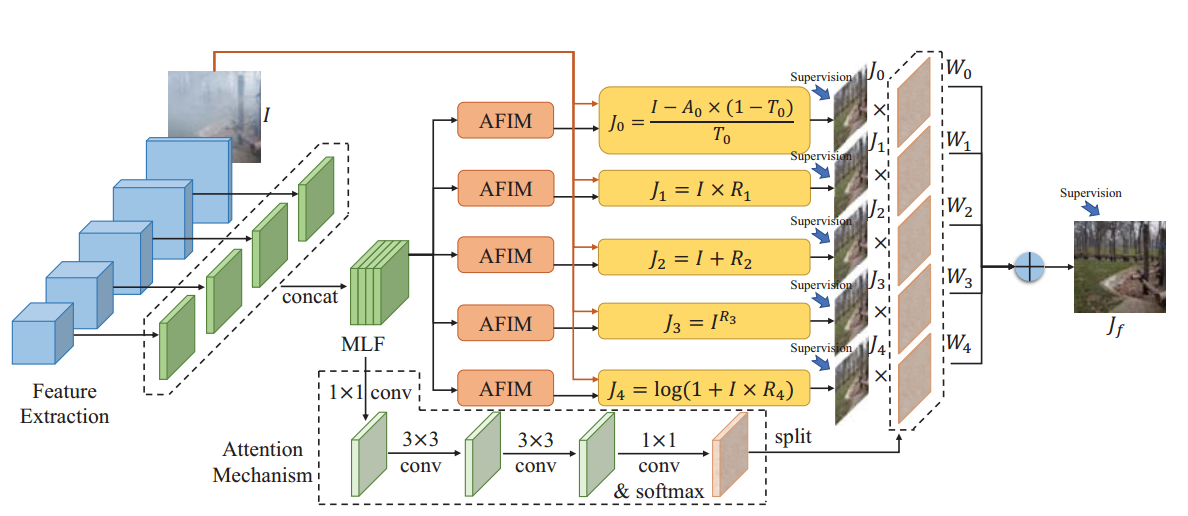
\includegraphics[width=.9\linewidth]{image/baseline_pip.png}
  \caption{DM2F算法流程图}
  \label{fig:fig2}
\end{figure*}

\subsubsection{效果评估}
作者与当时最先进的算法(sota)进行了比较,在多个数据集和多个指标的评估下,DM2F都达到了最优的效果。此外,对于最关键的多去雾模型融合的创新点,作者进行了多组充分的消融实验,结果表明,多去雾模型融合的效果要优于先前的光是依赖某个去雾模型的效果。

但是,我在复现论文时,发现了许多可改进的点。在OHaze数据集的测试结果表明,图像的细节存在模糊的情况;在HazeRD测试集上问题表现得更明显,模型难以广泛适用于不同浓淡的雾的去除。

\subsection{改进的算法}
针对两个测试集上的出现的问题,我采取了两种不同的算法分别进行改进。

在OHaze数据集上,为了保证恢复图像的高保真度,我引入了多色彩空间的细节增强网络,同时提出了高频低频信息分离的拉普拉斯损失。

在HazeRD数据集的效果改进上,我引入了GAN的对抗式训练并且加入了感知损失,同时根据训练完的判别器网络,在推理阶段使用重采样策略对未去雾完善的图像重复去雾。

\subsubsection{算法1:增强OHaze结果的图像细节}
受到计算机视觉领域多篇文献的启发,我想到了采用coarse-to-fine的策略,于是我构建了细节增强网络Detail Enhancing Network(DEN)。为了增强细节修复,我又引入了多色彩空间特征融合模块Multi-Color Fusion  (MCF),提出了拉普拉斯损失。

\begin{figure*}[t]
  \centering
  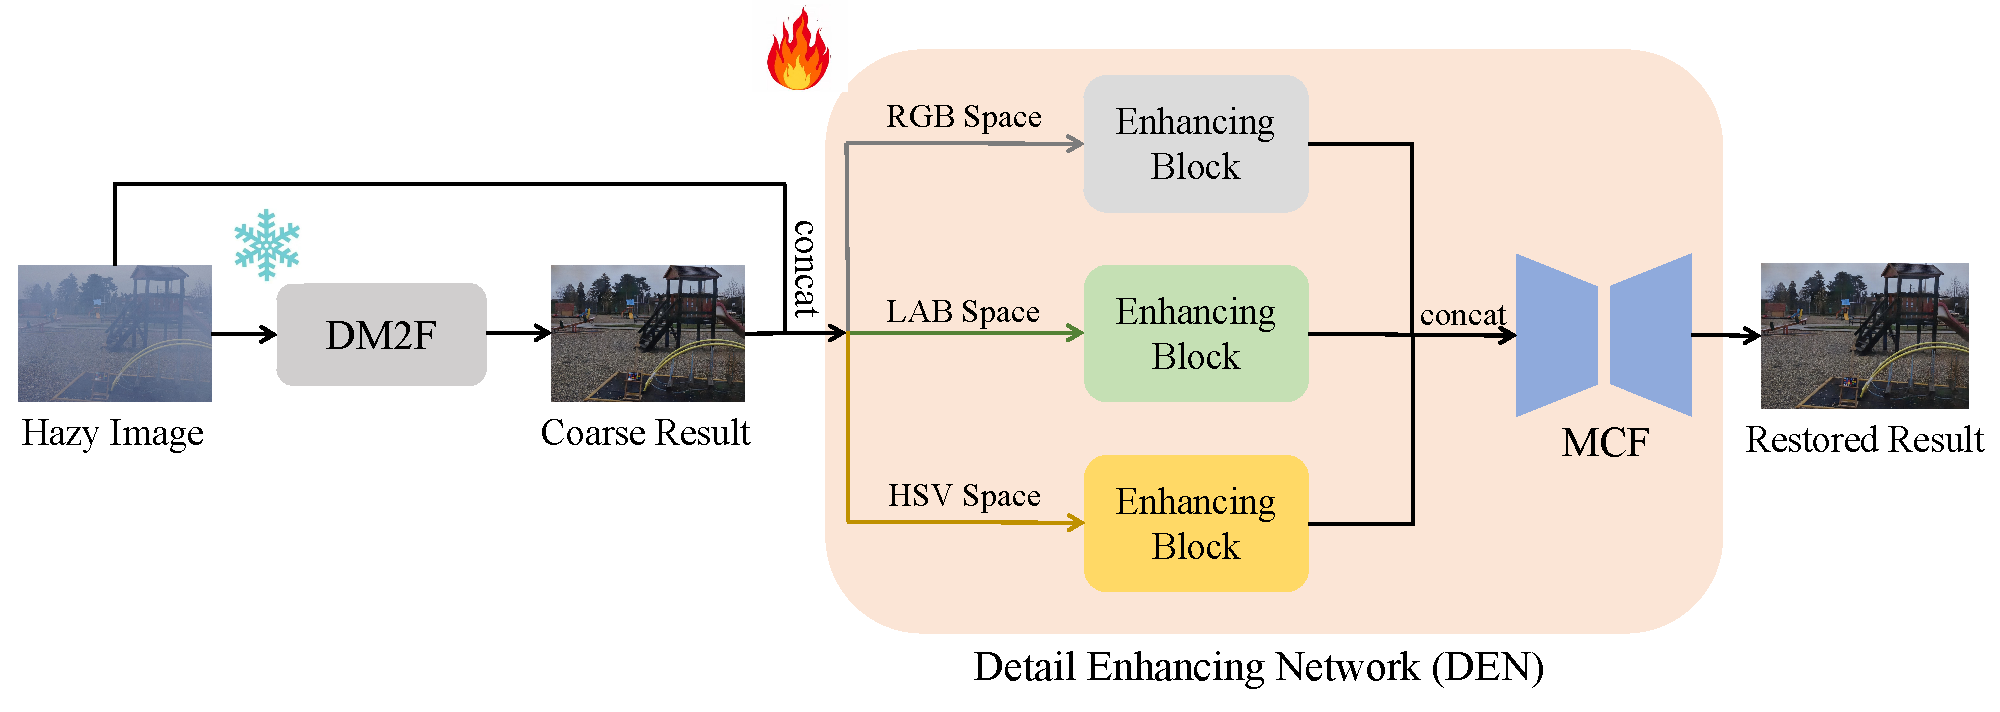
\includegraphics[width=.9\linewidth]{image/pip1.pdf}
  \caption{改进算法1的流程图}
  \label{fig:fig3}
\end{figure*}

\begin{figure*}[t]
  \centering
  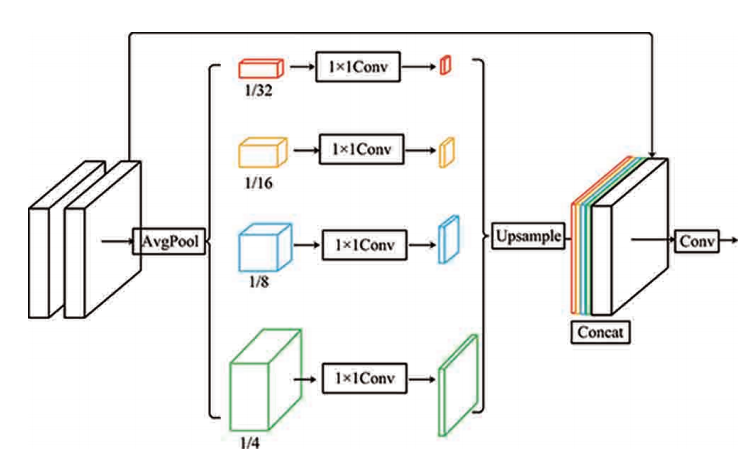
\includegraphics[width=.6\linewidth]{image/EB_pip.png}
  \caption{Enhancing Block的结构}
  \label{fig:fig4}
\end{figure*}


整个流程图见图\ref{fig:fig3},概述如下:
\begin{enumerate}
  \item 通过预训练的DM2F得到粗糙图像。
  \item 将粗糙图像与输入图像(含雾图像)拼接输入到DEN中。
  \item 将原始图像分别映射到三种色彩空间中提取特征,然后拼接。
  \item 将拼接完的特征输入到MCF中最终得到细节增强后的图像。
\end{enumerate}

实现细节:
\begin{itemize}
  \item 训练时我将DM2F参数冷冻,只训练细节增强网络的参数。
  \item Enhancing Block源自论文EPDN\cite{qu2019enhanced},见图\ref{fig:fig4}。
  \item MCF基于基础的UNet结构。
  \item 拉普拉斯损失(受到DocDiff\cite{yang2023docdiff}的启发):这是我自己命名的损失,旨在用拉普拉斯算子分离图像的高低频信息分别计算损失。具体计算方式见伪代码\ref{alg:cal_laplacian_loss}。
\end{itemize}

\begin{algorithm}
  \caption{Calculate Laplacian Loss}
  \label{alg:cal_laplacian_loss}
  \begin{algorithmic}[1]
  \REQUIRE Ground Truth $gt$, Prediction $pred$, Criterion $criterion$, Laplacian Operator $laplacian$
  \STATE $high\_pred \leftarrow laplacian(pred)$
  \STATE $low\_pred \leftarrow pred - laplacian(pred)$
  \STATE $high\_gt \leftarrow laplacian(gt)$
  \STATE $low\_gt \leftarrow gt - laplacian(gt)$
  \RETURN $criterion(high\_pred, high\_gt) + criterion(low\_pred, low\_gt)$
  \end{algorithmic}
  \end{algorithm}

\subsubsection{算法2:优化HazeRD多种浓度雾的去除效果}
为了解决HazeRD多浓度雾的去除问题,我主要在感知空间上下手。一,在原来损失函数的基础上引入了感知损失Perceptual Loss;二,为了使得生成图像更真实,使用GAN的对抗式训练来保证去雾后图像的真实性;三,在推理阶段,采用多次去雾的重采样策略,提升去雾效果。算法框架如图\ref{fig:fig5},下面详细介绍这三点改进。

\begin{figure*}[t]
  \centering
  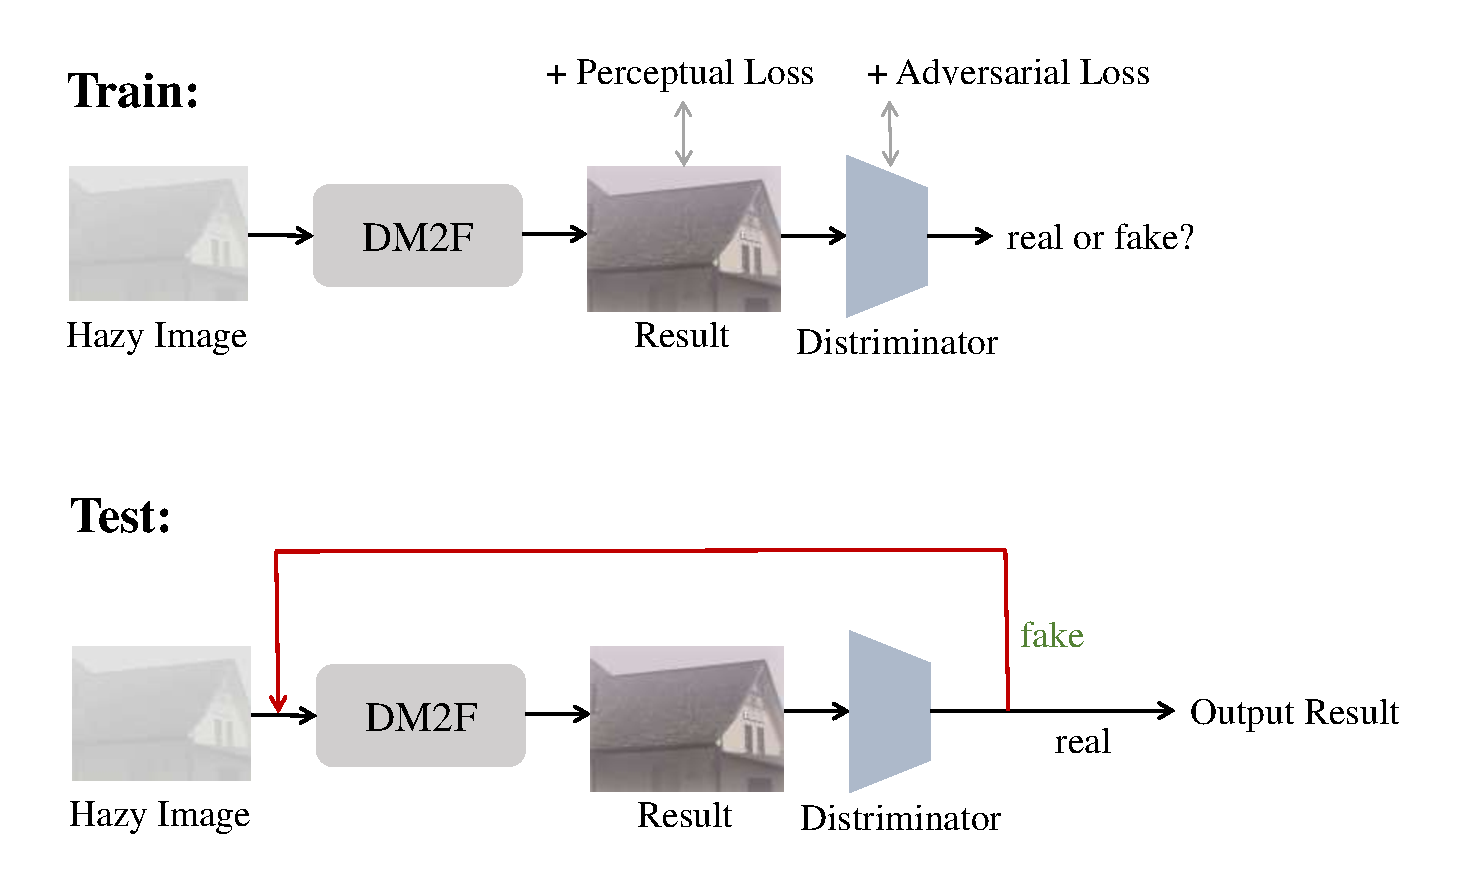
\includegraphics[width=.9\linewidth]{image/pip2.pdf}
  \caption{算法2的训练和测试流程图}
  \label{fig:fig5}
\end{figure*}

\textbf{感知损失}与传统的均方误差损失函数(Mean Square Error,MSE)相比,感知损失更注重图像的感知质量,更符合人眼对图像质量的感受。为了更好地保持感知和语义的保真度,本文中将原论文中的部分L1损失改成了这种损失。更具体地,我们从预训练的VGG网络中抽取多层的特征,激活后计算L1损失,公式如下:
\begin{equation}
  L_{VGG}(x, \hat{x}) = \sum_{i}{\frac{1}{C_iH_iW_i}}||\Phi_i(x) - \Phi_i(\hat{x})||_1
  \label{eq:perceptualloss}
\end{equation}
其中$\Phi_i$表示第i层特征的激活函数,$C_i, H_i, W_i$分别表示第i层特征的通道数、高度和宽度。$x$表示真实标签,$\hat{x}$表示模型的预测图像。

\textbf{对抗式训练}主要源自于GAN\cite{creswell2018generative}。其基本思想就是利用一个生成器和判别器的对抗,不断提升二者的能力,让生成器有足够的能力去骗过鉴别器。本文采用的是最基本的GAN的训练策略,其关键的一点就在于对抗损失Adversarial Loss,用数学公式描述如下:
\begin{equation}
  \mathbb{L}_A(G, D) = \mathbb{E}_{(X)} [\log D(X)] + \mathbb{E}_{(X)} [\log (1 - D(G(Y)))]
  \label{eq:adversarialloss}
\end{equation}
其中X表示无雾清晰图像,Y表示输入的带雾图像,G表示生成器,D表示判别器。具体在训练时,我们需要交替使得D和G的梯度下降,相当于$L_A = \min_{G} \left[ \max_{D} \mathbb{L}_A(\sim G, D) \right]$。最终消融实验表明,加入对抗式训练可以提高恢复图像质量和保真度。

\textbf{重采样策略}是我自己提出的策略,由于原先模型对浓雾的去除效果不够,于是直觉上来说多次去雾就可以优化去雾效果。我提出了如图\ref{fig:fig5}的推理流程,根据之前训练的判别器来判断是否去雾完全,如果去雾不完全就将结果重新送回网络重采样出去雾图像,直到最终图像能达到判别器的要求为止。

总之,算法2提出的三种策略结合起来,大大提高了HazeRD数据集上对不同程度的雾去除效果,会在后面实验部分具体分析。

\section{实验}

\subsection{实验启动}
\subsubsection{数据集介绍}
本文用到的数据集主要是OHaze\cite{ancuti2018haze}和HazeRD\cite{zhang2017hazerd}。此外还用到了RESIDE\cite{li2018benchmarking}数据集作为HazeRD的训练数据集。

OHaze是第一个引入的包含模糊和无烟雾(地面真实)图像的真实数据集。它由45个不同的户外场景组成,使用一个专业的雾霾发生器在控制照明下拍摄。本文采用前40张用作训练,后5张用作测试。

HazeRD 包含 15 个真实的室外场景,每个场景都模拟了五种不同的天气条件,所以测试集总共包含75张图像。HazeRD属于合成数据集,但能很大程度地模拟真实的雾天场景。

\subsubsection{实验设置}
在训练时,我们对OHaze数据做了预处理,将高分辨率图像crop成512x512的patches,作为模型输入。

在HazeRD的测试阶段,为了防止显存不足,我将原测试图像分辨率缩减了一半(通过下采样方法)。

算法1使用的DM2F的预训练参数是在OHaze上训练了20000轮的结果。

对于GAN的判别器的梯度下降,我们采用Adam优化器,其参数为$\beta_1 = 0.9, \beta_2 = 0.999$,初始学习率为5e-4。对于生成器的梯度下降,我们采用Adam优化器,其参数为$lr_{decay}=0.9$,初始学习率为5e-4。
\subsubsection{指标介绍}

本文采用四个指标来评价去雾效果,分别为PSNR, SSIM, CIEDE2000和MSE。
\begin{itemize}
    \item PSNR是评价图像质量的一种常用指标,它衡量了原始图像与重建图像之间的峰值信噪比。PSNR的数值越高,表示图像质量越好。
    \item SSIM是一种评价图像相似性的指标,它考虑了亮度、对比度和结构三个方面的信息。SSIM数值越接近1表示图像相似性越高。
    \item CIEDE2000是一种颜色差异评价指标,用于比较两个颜色之间的感知差异。它考虑了颜色的亮度、饱和度和色调等因素。数值越小表示图像相似度越高。
    \item MSE是衡量两个图像之间差异的一种度量标准。它计算了原始图像和重建图像之间每个像素的差异的平方,并对所有差异进行平均。MSE越小,表示图像之间的差异越小,重建图像与原始图像之间的接近程度越高。
\end{itemize}


\subsection{与Baseline效果对比}

为了验证改进算法1和改进算法2的有效性,我分别在两个指定数据集上测试了模型的去雾效果,从可视化效果和量化指标结果两个方面来验证算法的性能。

\begin{table}[!htb]
  \centering
  \caption{改进算法1与Baseline在OHaze数据集上的定量效果对比。
  Baseline(Paper)表示原论文中的指标,Baseline(Code)表示我复现的指标。}
  \label{tab:1}
  \small % 缩小表格字体
  % \setlength{\tabcolsep}{4pt} % 调整列之间的宽度
  % \begin{adjustbox}{width=\textwidth,center}
  \scalebox{1.}{
  \begin{tabular}{lcccc} 
  \toprule
  Method & PSNR↑ & SSIM↑ & CIEDE2000↓ & MSE(\%)↓ \\
  \midrule
  \textbf{Baseline(Paper)} & 25.188 & 0.777 & - & - \\
  \textbf{Baseline(Code)} & 25.114 & 0.773 & 5.106 & 0.960 \\
  \textbf{Ours} & \textbf{25.234} & \textbf{0.786} & \textbf{5.014} & \textbf{0.937}  \\
  \bottomrule
  \end{tabular}}
  % \end{adjustbox}
  \end{table}

算法1与Baseline在OHaze上测试,虽然从可视化角度难以区分效果优劣,但是在指标上,改进算法1优于原始算法,由此说明在多色彩空间上对于图像细节的增强对于指标的提升有作用。定量指标评估结果见表\ref{tab:1}。

算法2与Baseline在HazeRD的不同浓度雾的场景图像上测试,单从可视化角度评估,改进算法就明显优于原算法,从图\ref{fig:fig6}中明显看到改进算法2的去雾效果显著,不会像原算法一样对浓雾情况无效,这是因为加入了感知空间的损失函数并且使用了对抗式训练策略。从表\ref{tab:2}的定量评估指标来看,改进算法2也远超原始算法。

  \begin{figure*}[t]
    \centering
    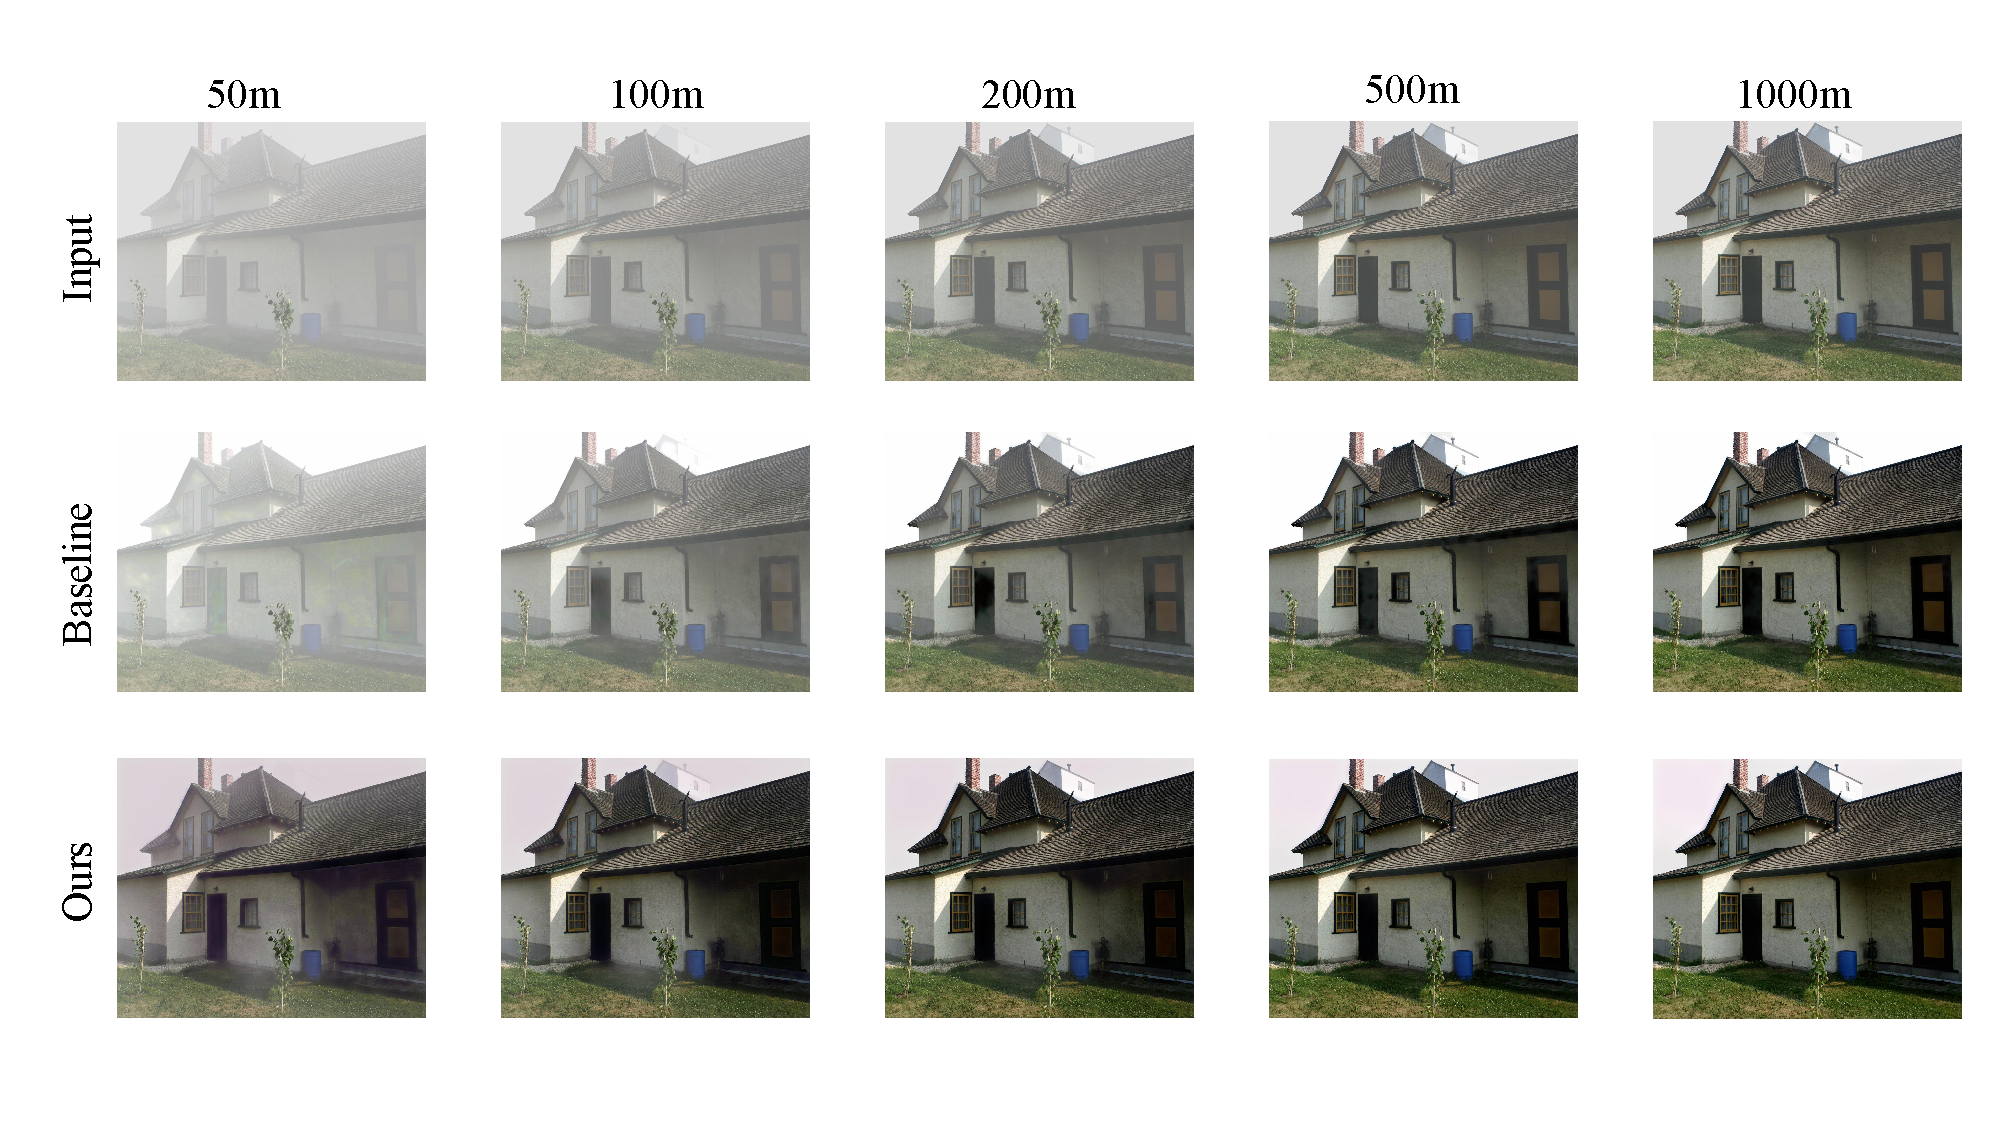
\includegraphics[width=.9\linewidth]{image/fig2.pdf}
    \caption{算法2和Baseline在HazeRD的不同能见度雾下的去雾可视化效果图}
    \label{fig:fig6}
  \end{figure*}


  \begin{table}[!htb]
    \centering
    \caption{改进算法2与Baseline在HazeRD数据集上的定量效果对比。}
    \label{tab:2}
    \small % 缩小表格字体
    % \setlength{\tabcolsep}{4pt} % 调整列之间的宽度
    % \begin{adjustbox}{width=\textwidth,center}
    \scalebox{1.}{
    \begin{tabular}{lcccc} 
    \toprule
    Method & PSNR↑ & SSIM↑ & CIEDE2000↓ & MSE(\%)↓ \\
    \midrule
    \textbf{Baseline(Paper)} & - & 0.656 & 12.9285 & - \\
    \textbf{Baseline(Code)} & 13.588 & \textbf{0.779} & 17.3398 & 23.93 \\
    \textbf{Ours} & \textbf{15.939} & 0.749 & \textbf{14.4298} & \textbf{8.45} \\
    \bottomrule
    \end{tabular}}
    % \end{adjustbox}
    \end{table}

\subsection{消融实验}
算法1的消融:从Baseline出发,逐步加入Enhancing Block,多色彩空间融合(MCF),拉普拉斯损失的对比效果如表\ref{tab:3}所示。可以看到只使用简单的Refinement网络时,去雾效果反倒会变差,在加入多色彩空间特征融合模块和拉普拉斯损失之后,效果都有提升。

算法2的消融:从Baseline出发,逐步加入感知损失、GAN的对抗式训练、重采样策略的对比效果如表\ref{tab:4}所示。可以看到GAN对效果提升最为显著,其余两个策略都有小幅提升。

\begin{table}[!htb]
  \centering
  \caption{改进算法1的消融实验效果表}
  \label{tab:3}
  \small % 缩小表格字体
  % \setlength{\tabcolsep}{4pt} % 调整列之间的宽度
  % \begin{adjustbox}{width=\textwidth,center}
  \scalebox{1.}{
  \begin{tabular}{ccc|cccc} 
  \toprule
  Enhancing Block & MCF & Laplacian Loss & PSNR↑ & SSIM↑ & CIEDE2000↓ & MSE(\%)↓ \\
  \midrule
  & & & 25.114 & 0.773 & 5.106 & 0.960 \\
  $\checkmark$ & & & 25.104 & 0.784 & 5.200 & 0.964 \\
  $\checkmark$ & $\checkmark$ & & 25.205 & \textbf{0.788} & \textbf{4.992} & 0.943 \\
  $\checkmark$ & $\checkmark$ & $\checkmark$ & \textbf{25.234} & 0.786 & 5.014 & \textbf{0.937} \\
  % \textbf{Baseline(Code)} & 13.588 & \textbf{0.779} & 17.3398 & 23.93 \\
  % \textbf{Ours} & \textbf{15.939} & 0.749 & \textbf{14.4298} & \textbf{8.45} \\
  \bottomrule
  \end{tabular}}
  % \end{adjustbox}
  \end{table}

  \begin{table}[!htb]
    \centering
    \caption{改进算法2的消融实验效果表}
    \label{tab:4}
    \small % 缩小表格字体
    % \setlength{\tabcolsep}{4pt} % 调整列之间的宽度
    % \begin{adjustbox}{width=\textwidth,center}
    \scalebox{1.}{
    \begin{tabular}{ccc|cccc} 
    \toprule
    Perceptual Loss & GAN & Resampling & PSNR↑ & SSIM↑ & CIEDE2000↓ & MSE(\%)↓ \\
    \midrule
    & & & 13.588 & 0.779 & 17.3398 & 23.93 \\
    $\checkmark$ & & & 14.778 & \textbf{0.798} & 16.5095 & 20.13 \\
    $\checkmark$ & $\checkmark$ & & 15.646 & 0.756 & \textbf{14.0306} & 9.33 \\
    $\checkmark$ & $\checkmark$ & $\checkmark$ & \textbf{15.939} & 0.749 & 14.4298 & \textbf{8.45} \\
    % \textbf{Baseline(Code)} & 13.588 & \textbf{0.779} & 17.3398 & 23.93 \\
    % \textbf{Ours} & \textbf{15.939} & 0.749 & \textbf{14.4298} & \textbf{8.45} \\
    \bottomrule
    \end{tabular}}
    % \end{adjustbox}
    \end{table}

\subsection{自己搜集的图片集上的实验}
我在互联网上搜集了5张室外场景的雾天图像,利用改进算法进行了去雾处理,可视化效果如图\ref{fig:fig7}。

\begin{figure*}[t]
  \centering
  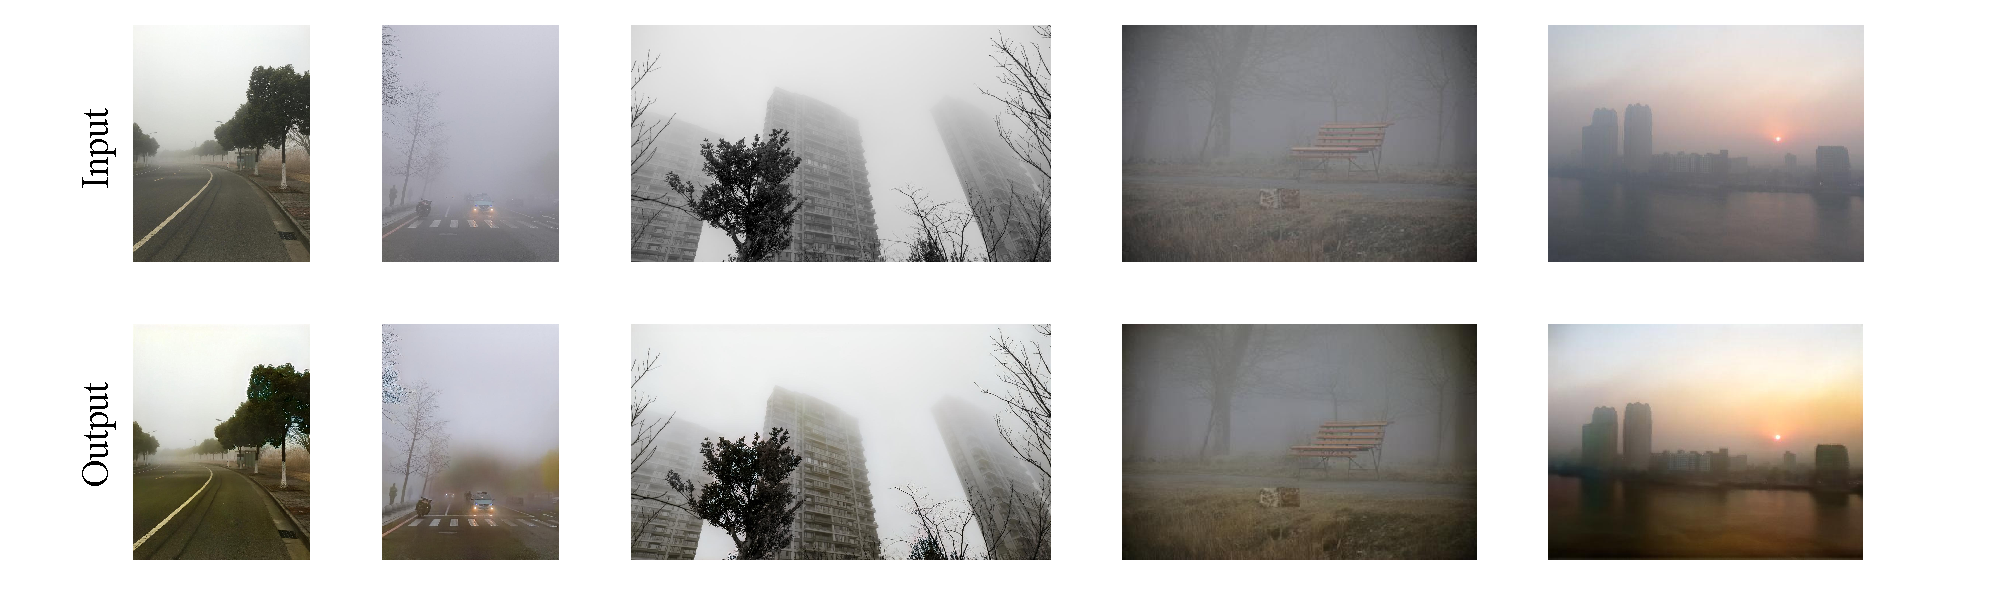
\includegraphics[width=.9\linewidth]{image/pic3.pdf}
  \caption{在自己搜集的图片集上的去雾可视化效果图}
  \label{fig:fig7}
\end{figure*}



\section{结论}

针对单幅图像去雾问题,本文总结和分析了过去的传统算法和基于深度学习的算法的优劣。在DM2F作为Baseline模型的基础上,发现其存在的图像细节模糊、难以适应多浓度雾的去除这两个关键问题。对于这两个问题针对性地改进了两种算法。算法1采用coarse-to-fine的思路,创新性地提出了多色彩空间特征融合的细节增强网络,同时加入拉普拉斯损失进一步提升了去雾效果;算法2考虑从感知空间入手,引入感知损失和GAN的对抗式训练,并利用预训练好的判别器在推理阶段使用了重采样策略来提升浓雾的去除效果。我进行了充分的比较实验和消融实验,多个数据集上的多组指标对比实验以及可视化结果表明,我提出的各个模块都有效果的提升,提出的两个改进算法在去雾效果上都比Baseline更优越。

\section{感悟}
\begin{itemize}
  \item 现在许多深度学习算法都专注于对于模块、网络结构的研究,而忽视了传统算法中对于图像本身性质的提取方法、研究策略等,本文发现传统算法中的拉普拉斯算子、图像的多色彩空间等策略能在深度学习算法的改进中起到不小的作用。
  \item 本文存在的缺陷:无法同时顾及细节增强和多浓雾去除,换句话说,改进算法1和改进算法2融合起来的效果并不好;此外,利用多色彩空间的算法可能会导致出现某些错误的颜色块。
\end{itemize}

\bibliography{cite}





\end{document}